\chapter{Programme}\label{chap:programme2}
Im Mittelpunkt dieser Bachelorarbeit steht \gls{seapp}, welches auf \gls{omnetpp} mit \gls{inet} aufbaut. Im Folgenden werden diese zentralen Programme vorgestellt. Zuerst wird auf \gls{omnetpp} erweitert mit \gls{inet} als Kernkomponente eingegangen. Danach wird \gls{seapp} vorgestellt, welches  Angriffssimulationen auf \gls{omnetpp}-Topologien ermöglicht.

\section{\glsentryname{omnetpp} und \glsentryname{inet}}
\gls{omnetpp} ist eine in C++ geschriebene Event-Simulationsplattform. Zusätzlich zu dem eigentlichen Simulationskern bietet \gls{omnetpp} eine Eclipse-\gls{ide}. Topologien werden in einer \gls{dsl}, \gls{ned} genannt, definiert. \cite{OMNeTOverview}

Um Computernetzwerke darzustellen wird \gls{omnetpp} mit \gls{inet} erweitert. Die Erweiterung \gls{inet} bietet viele Implementierungen von Netzwerkprotokollen und -geräten an, wie \zB einen Switch oder Router. 

\subsection{Die \glsentryname{ned}-Sprache} 
\begin{figure}
	\centering
	\includestandalone[keepaspectratio]{tikz/baExampleTop}
	\caption[Beispieltopologie]{Beispieltopologie definiert in \ref{lst:exampleNed}}
	\label{fig:exampleTopologie}
\end{figure}
Zuerst soll auf die \gls{ned}-Sprache anhand eines Beispiels eingegangen werden. Die Beispieltopologie \ref{lst:exampleNed} besteht aus drei Akteuren Alice, Bob und Eve, welche über einen Router kommunizieren können. Eine grafische Darstellung findet sich in der Abbildung \ref{fig:exampleTopologie}, welche nur Netzwerkmodule darstellt.

\subsubsection{Beispielimplementierung in der \glsentryname{ned}-Sprache}
\begin{program}[ht]
	\lstinputlisting[firstline=10, language=NED, caption={[Beispiel NED-Definition]}]{listings/example.ned}
	\caption[Beispiel NED-Definition]{Auszug aus dem \gls{ned} Beispiel für die in Abbildung \ref{fig:exampleTopologie} dargestellte Topologie.}
	\label{lst:exampleNed}
\end{program}
Um den Aufbau von Topologien in \gls{omnetpp} nachzuvollziehen, sind einige \gls{omnetpp}-spezifische Begriffe zu klären. \gls{omnetpp}-Simulationen werden aus Knoten (Nodes) und Kanälen (Channel) aufgebaut. Knoten sind im ersten Beispiel \ref{lst:exampleNed} die Elemente \ned{alice, bob, eve, router}. Die Verbindungen zwischen den Knoten repräsentieren die Kanäle.

Knoten werden intern als Module umgesetzt. Module können weiter unterschieden werden in zusammengesetzte (compound modules) und einfache Module (simple modules).

Ein einfaches Modul stellt durch eine Implementierung in \gls{c++} grundlegende Funktionalitäten zur Verfügung. Es ist für das Aufzeichnen von Statistiken verantwortlich. Komplexere Strukturen, wie zum Beispiel ein Switch, können dann durch einen Zusammenschluss von mehreren einfachen Modulen ohne \gls{c++}-Code realisiert werden \cite{OmnetBirdsEye2020}. Zusätzlich zu den Modulen existieren Interfaces, welche von Modulen realisiert werden können \cite[\absatz{3.1}]{OmnetManual}. 

In \gls{omnetpp} wird intern jedem Modul eine \ned{id} zugewiesen, welche für die Zeit der Simulation  garantiert einzigartig ist \cite[\absatz{4.11}]{OmnetManual}. In dieser Arbeit werden keine neuen Module erstellt, sondern nur vorhandene konfiguriert und in einer Topologie implementiert.

In dem gekürzten Quellcode\footnote{Die Beispieltopologie lässt einige Details aus. In den ausgelassenen Zeilen wird ähnlich zu Java ein \ned{package} festgelegt und vorgefertigte Modulen geladen. Wenn diese Zeilen inkludiert werden, wird das Beispiel zu lang für die Darstellung auf dieser Seite.} in Zeile 1 wird ein neues Netzwerk mit dem Namen \ned{Example} erstellt. Ein Netzwerk ist das Modell, welches simuliert werden soll und ist selbst ein Modul \cite[\absatz{2.1}]{OmnetManual}.

Ein \gls{omnetpp}-Modul kann die Abschnitte \ned{types, parameters, gates, submodules} und \ned{connections} beinhalten \cite[\absatz{3.4}]{OmnetManual}, wobei das Beispielnetzwerk drei dieser Abschnitte nutzt. In dem Parameterabschnitt können Variablen definiert und zugewiesen werden. In diesem Beispiel ist es ein \ned{string attackConfigurationFile}\footnote{Der String \ned{attackConfigurationFile} enthält die Angriffsbeschreibung für \gls{seapp}.} mit einem leeren Wert \ned{default}.

Unter \ned{submodules} werden die genutzten Module definiert \cite[\absatz{3.4}]{OmnetManual}. In Beispielquellcode sind \ua \ned{alice, bob, eve} Module des Typs \ned{StandardHost}, welche mit einer späteren Konfiguration Dienste in dem Netzwerk bereitstellen.

Zuletzt nutzt das Beispiel den \ned{connections} Abschnitt, in welchen Verbindungen zwischen den Modulen, mithilfe von Kanälen, hergestellt werden \cite[\absatz{3.4}]{OmnetManual}. 

In dem Quellcode wird \zB eine Verbindung zwischen dem \ned{router} und den Rechnern \ned{alice, bob, eve} über ein \ned{Eth1G} Kanal hergestellt. Dieser Kanal ist ein Modell eines 1-Gigabit-Ethernetkabels. Die Option \ned{allowunconnected}, teilt \gls{omnetpp} mit, dass nicht alle Gates verbunden sein müssen. Ein Gate ist dabei, der Kommunikationsendpunkt zwischen Modulen.

\subsubsection{Weitere \glsentryname{ned}-Details}
Die nicht genutzten Abschnitte \ned{type} und \ned{gates} werden vor allem für Module in unteren Hierarchieebenen wichtig.

In dem \ned{type}-Abschnitt werden lokale Module und Kanäle definiert und im \ned{gates}-Abschnitt Ports, die in \gls{omnetpp} Gates genannt werden \cite[\absatz{3.4}]{OmnetManual}. Diese erlauben die Kommunikation zwischen den einzelnen Modulen. In dem Beispielquellcode besitzt das Modul \ned{StandardHosts} zwei Gates mit den Namen \ned{ethg} und \ned{global\_filter}. Der \ned{globalFilter} besitzt ein Gate mit dem Namen \ned{nodes}.

Für die Gates wird ein weiteres, aus Programmiersprachen bekanntes Feature verwendet. In \gls{ned} ist es möglich Vektoren (Arrays) zu definieren, um \zB eine über ein Parameter skalierbare Anzahl an Modulen eines spezifischen Typs zu erzeugen oder mehrere Schnittstellen zu anderen Modulen über Gates anzubieten. In dem Quellcode hätten die drei \ned{StandardHost} durch \ned{host[anzahl]: StandardHost} dargestellt werden können, wobei \ned{anzahl} einen Integerwert entspricht. Für die Vektoren unterstützt \gls{ned} Schleifen. Bei den Gates wird durch die Notation \ned{++} ein nicht genutztes Feld des Vektors \ned{ethg} referenziert. \cite[\absatz{3}]{OmnetManual} Diese Sprachfunktionalität wird im Beispiel genutzt, um den Router mit den Hosts zu verbinden, ohne konkret die Felder \ned{ethg[0],ethg[1]} und \ned{ethg[2]} referenzieren zu müssen.

\subsection{Wichtige \glsentryname{inet}-Module}
Im folgenden werden alle für diese Arbeit genutzten Module vorgestellt. Bereits bekannt sind die Module \ned{StandardHost} \ref{fig:standardHost} und \ned{Router} \ref{fig:router}. Zusätzlich sollen die Module \ned{EtherSwitch} \ref{fig:switch} und \ned{InternetCloud} \ref{fig:inetCloud} betrachtet werden.

\begin{figure}[ht]
	\centering
	\begin{subfigure}{0.5\textwidth}
		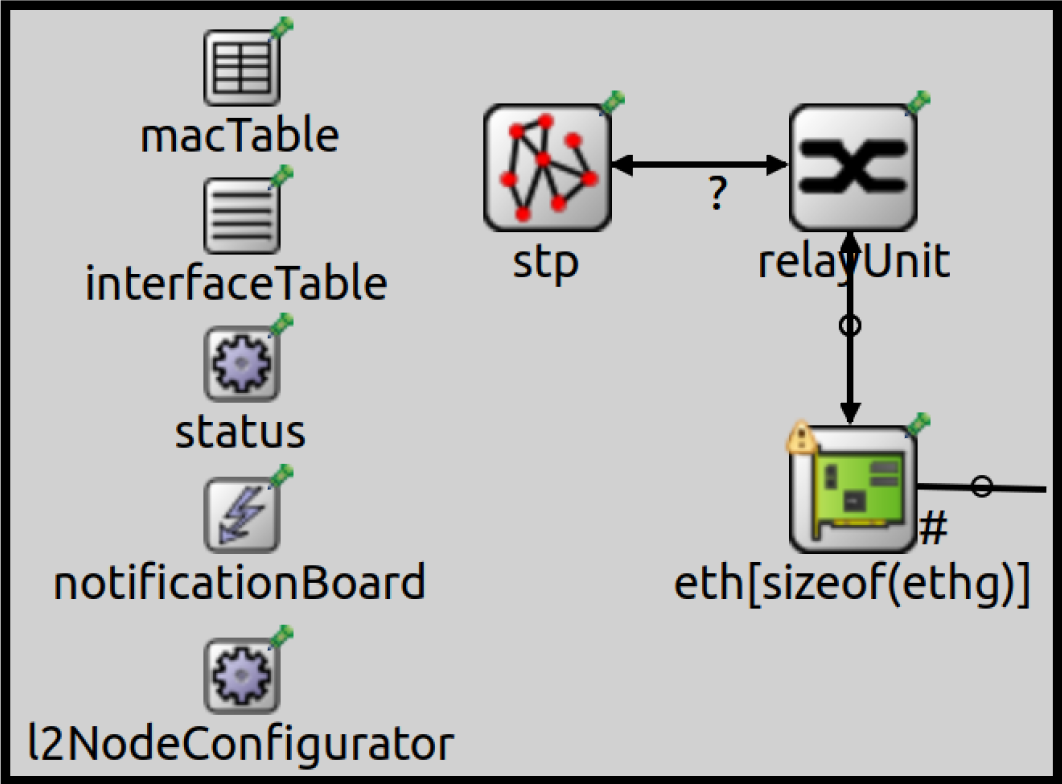
\includegraphics[width=0.7\linewidth, height=5cm, keepaspectratio]{pic/EthernetSwitch}
		\caption[EthernetSwitch]{EthernetSwitch} 
		\label{fig:switch}
	\end{subfigure}%
	\begin{subfigure}{0.5\textwidth}
		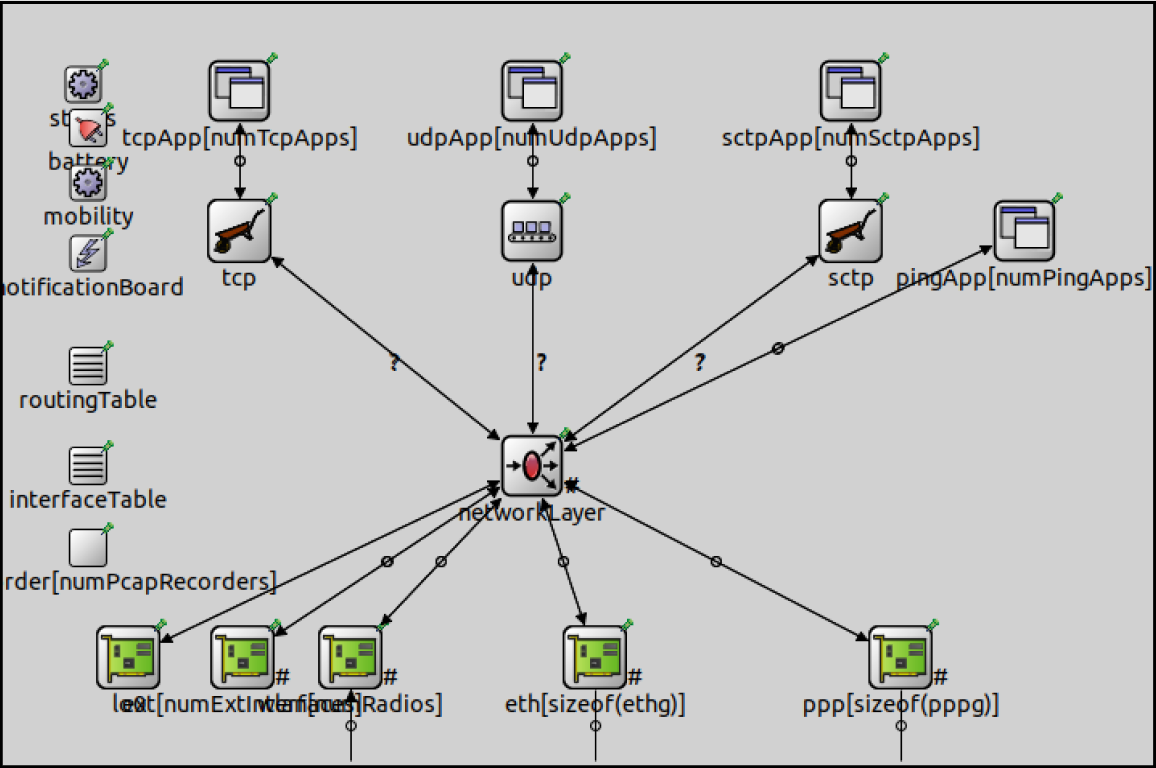
\includegraphics[width=0.7\linewidth, height=5cm, keepaspectratio]{pic/StandardHost}
		\caption[StandardHost]{StandardHost} 
		\label{fig:standardHost}
	\end{subfigure}
	\begin{subfigure}{0.5\textwidth}
		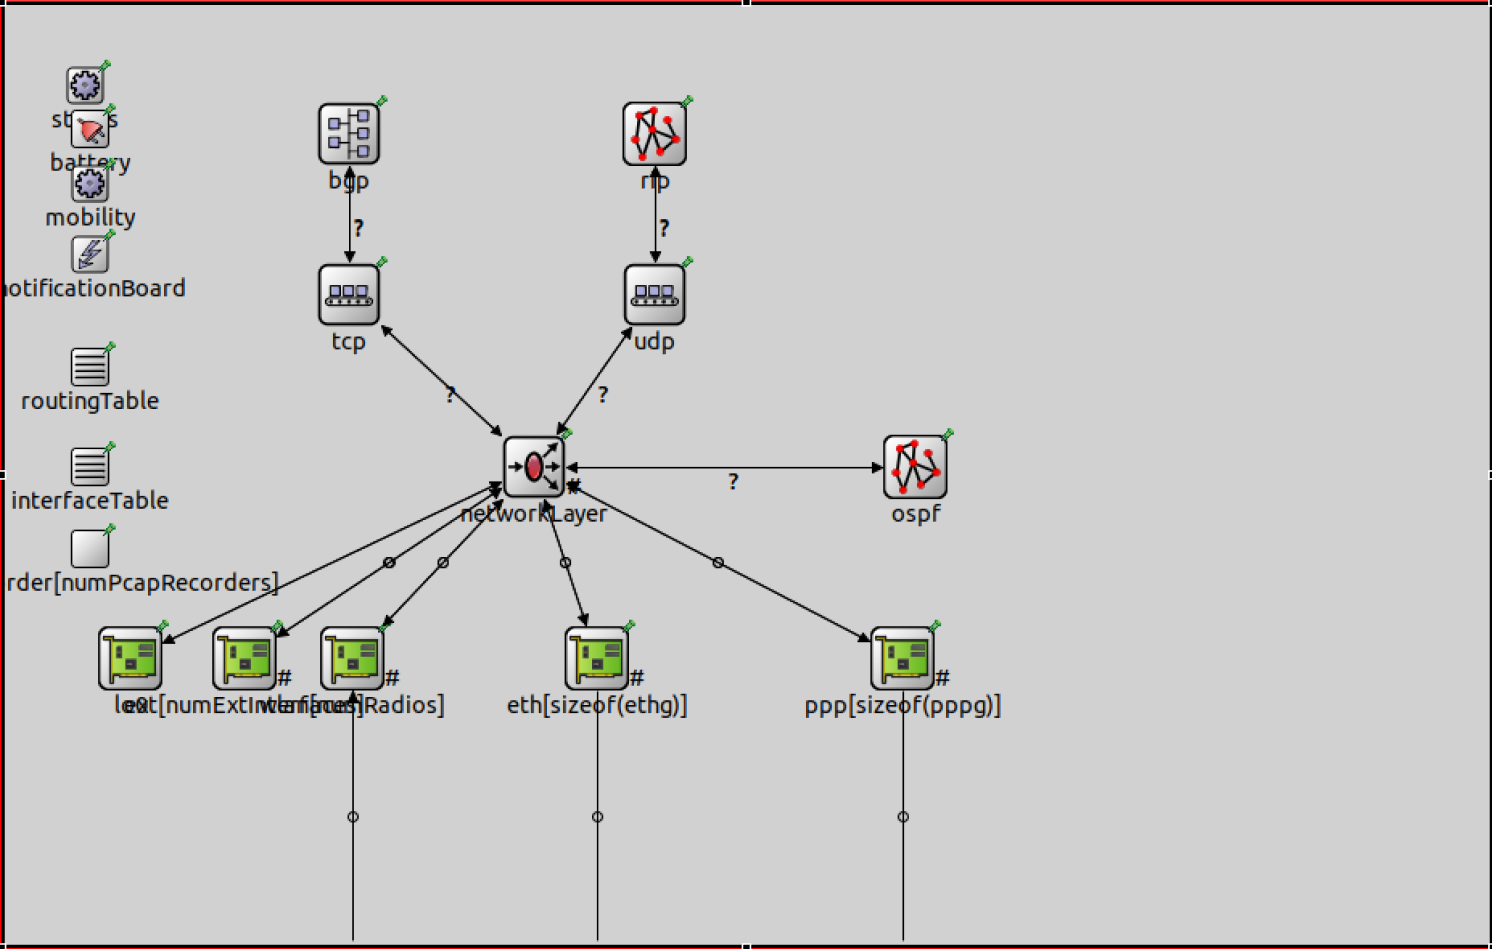
\includegraphics[width=0.7\linewidth, height=5cm, keepaspectratio]{pic/Router}
		\caption[Router]{Router} 
		\label{fig:router}
	\end{subfigure}%
	\begin{subfigure}{0.5\textwidth}
		\includegraphics[width=0.7\linewidth, height=5cm, keepaspectratio]{pic/internetCloud}
		\caption[InternetCloud]{InternetCloud} 
		\label{fig:inetCloud}
	\end{subfigure}
	\caption[Wichtige Module]{\gls{omnetpp}-Ansicht der genutzten Module}
	\label{fig:usedModules}
\end{figure}

Für die Angriffe auf ein Netzwerk, wird die Erweiterung \gls{seapp} \ref{sec:seapp} benutzt. Diese Erweiterung benötigt das Modul \ned{LocalFilter} in jedem Modul mit welchem \gls{seapp} zur Laufzeit interagiert. Da \gls{seapp} keine Integration in die Eclipse-\gls{ide} bietet, wurde dieses Modul in Abbildung \ref{fig:usedModules} nicht dargestellt.

\begin{table}[ht]
	\centering
	\begin{tabularx}{\textwidth}{|c|X|}
		\hline
		\rowcolor{Gainsboro!60}
		            Modul             & Beschreibung                                                                               \\ \hline
		\ned{IPv4NetworkConfigurator} & Konfiguriert IP-Adressen und statisches Routing im IPv4-Netzwerk                           \\ \hline
		       \ned{EtherMAC}         & Setzt \gls{layer2} Funktionen um. Unterstützt IEEE 802.3.                                \\ \hline
		     \ned{ThruputMeter}       & Zeichnet Anzahl und Durchsatz für ein- und ausgehende Datenpakete auf. \\ \hline
		\ned{ARP,TCP,UDP} und weitere & Implementierungen der jeweiligen Protokolle                                                \\ \hline
	\end{tabularx}
	\caption[Beschreibung wichtiger Module]{Kurzbeschreibung wichtiger einfacher Module}
	\label{table:einfacheModule}
\end{table}

Die Funktionen der wichtigsten einfachen Module sind in der Tabelle \ref{table:einfacheModule} beschrieben. Zusammengesetze Module wie \zB \ned{L2NodeConfigurator} oder \ned{InterfaceTable} wurden ausgelassen, da diese beim späteren Konfigurationsprozess nicht benutzt werden. Die Implementierungsdetails sind jeweils aus der Dokumentation in den \ned{.ned}-Dateien entnommen, da diese den Entwicklungsstand für die jeweilige \gls{inet}-Version beschreiben. Zusätzlich finden sich in dieser Datei die Statistiken und Signale, welche von den einfachen Modulen aufgezeichnet werden sowie die Analyse des Modells erlauben.

\begin{figure}[ht]
	\centering
	\begin{subfigure}{0.5\textwidth}
		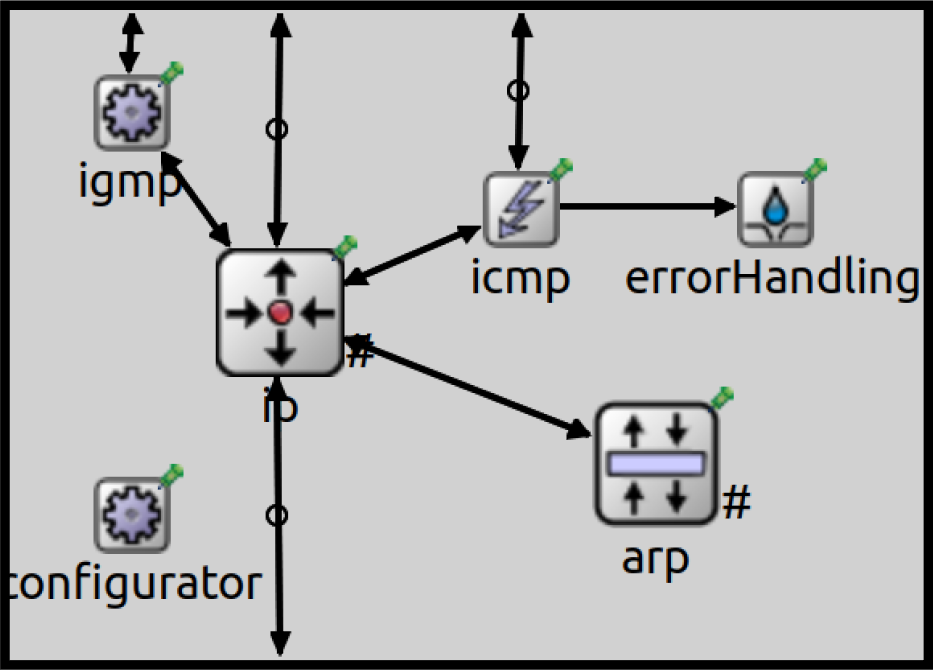
\includegraphics[width=0.7\linewidth, height=5cm, keepaspectratio]{pic/NetworkLayer}
		\caption[EthernetInterface]{NetworkLayer} 
		\label{fig:networkLayer}
	\end{subfigure}%
	\begin{subfigure}{0.5\textwidth}
		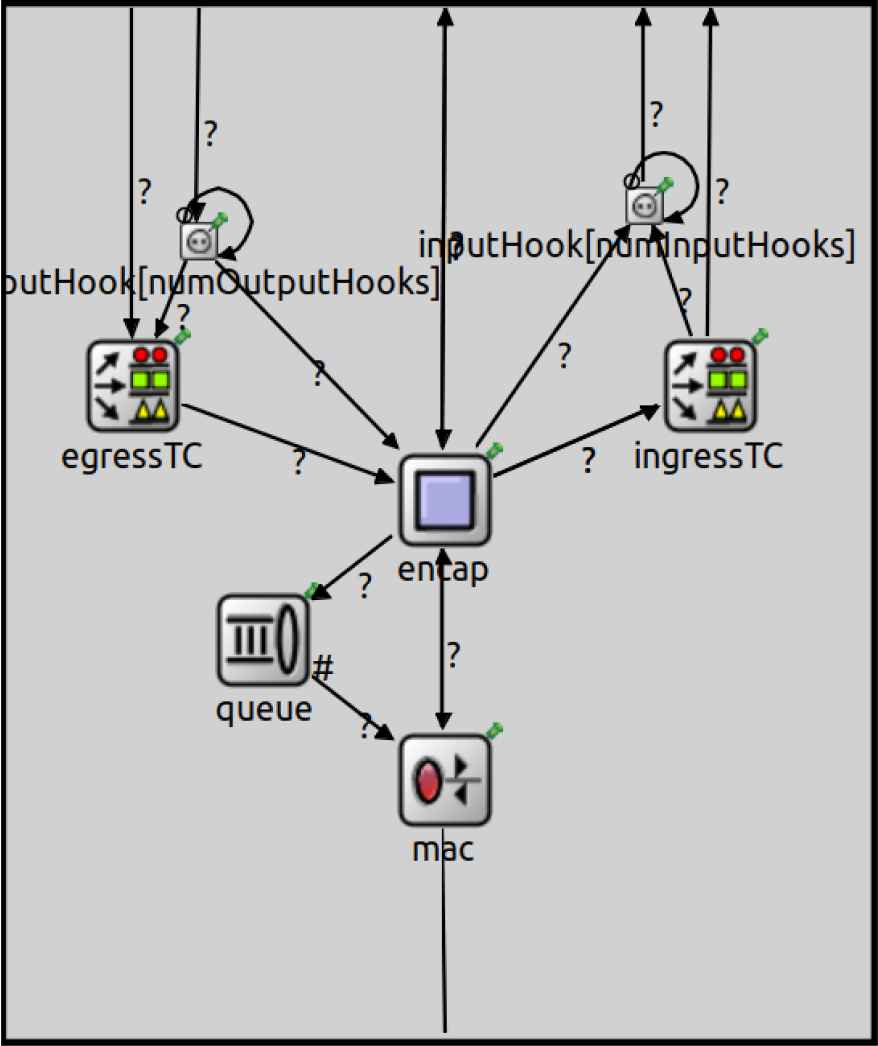
\includegraphics[width=0.7\linewidth, height=5cm, keepaspectratio]{pic/EthernetNic}
		\caption[Networklayer]{EthernetInterface} 
		\label{fig:EthernetInterface}
	\end{subfigure}
	\caption[Networklayer und EthernetInterface]{\gls{omnetpp}-Ansicht implizit genutzter zusammengesetzer Module}
\end{figure}

Zusätzlich zu den einfachen Modulen werden die zusammengesetzten Module \ned{NetworkLayer} \ref{fig:networkLayer} und \ned{EtherNic} \ref{fig:EthernetInterface} von den vorgestellten Netzwerkgeräten verwendet.

\subsubsection{\ned{EthernetInterface}}
Um ein Ethernet \gls{nic} zu realisieren, ist das zusammengesetzte Modul \ned{EthernetInterface} (\ref{fig:EthernetInterface}) in allen betrachteten Modulen, außer der \ned{InternetCloud}, welche ein ähnliches Modul für \gls{ppp}-Verbindungen verwendet, vorhanden. Es besteht aus Implementierungen der Modulinterfaces \ned{IHook, IEtherMAC, ITrafficConditioner} und \ned{IWiredNic} sowie einem zusammengesetzten Modul \ned{EtherQoSQueue}.

Das \ned{EthernetInterface} Modul ist dabei wie folgt konfiguriert. Es verwendet das Modul \ned{EtherMAC}, als Implementierung von \ned{IEtherMAC}. Das Interface \ned{IHook} wird von dem \ned{ThruputMeter} realisiert. Das Interface \ned{ITrafficConditioner} wird für QoS-Netzwerke benötigt und bleibt in dieser Arbeit außen vor. 

Das zusammengesetzte Modul \ned{EtherQoSQueue} implementiert Queues, und kann mit einer \ned{DropTailQueue} belegt werden.

\subsubsection{\ned{Networklayer}}
Das Modul \ned{Networklayer} (\ref{fig:networkLayer}) besteht aus den einfachen Modulen \ned{IPv4, IPv4NodeConfigurator\footnote{In der bildlichen Darstellung (\ref{fig:networkLayer}) werden Variablennamen angezeigt und nicht die Namen der Module. Beispielsweise wird der \ned{IPv4NodeConfigurator} nur als \ned{configurator} angezeigt.}, ARP, ICMP, IGMP} und \ned{ErrorHandling}. Diese Module setzten ihrem Namen entsprechend die grundlegenden Netzwerkprotokolle \gls{ipv4}, \gls{arp}, \gls{icmp} und \gls{igmp} um, welche für die Kommunikation auf der \gls{layer3} wichtig sind.


\subsubsection{\ned{EtherSwitch}}
Der Begriff des Switches wird in realen Netzwerken für \gls{layer2}- und \gls{layer3}netzwerkgeräte verwendet. In \gls{omnetpp} wird ein Modul für die \gls{layer2}-Switch Funktionalität definiert. Die Abbildung \ref{fig:switch} zeigt grafisch den Aufbau eines Switches in \gls{omnetpp}. Das Modul besteht aus den einfachen Modulen \ned{L2NodeConfigurator, InterfaceTable, NotificationBoard, MACAddressTable, MACRelayUnit} und optional einer Implementierung des \ned{ISpanningTree}. Im Gegensatz zu Modulen auf Basis des Moduls \ned{NodeBase} besitzt der \file{EtherSwitch.ned} kein Gate für den \ned{GlobalFilter}. Dies schränkt den Einsatz mit \gls{seapp}\footnote{Die Bedeutung des \ned{GlobalFilter} wird im Abschnitt \ref{sec:seapp} erklärt.} ein.



\subsubsection{\ned{StandardHost} und \ned{Router}}
Die Module \ned{StandardHost} und \ned{Router} erben von dem Modul \ned{NodeBase}, weshalb deren interner Aufbau ähnlich ist. Das Grundmodul \ned{NodeBase} ist in der \file{NodeBase.ned} definiert und bietet die Grundlage für Ethernet, \gls{ppp} und Wireless-Verbindungen an. Dies inkludiert das zusammengesetztes Modul \ned{Networklayer}, welches einfache Module zur IP-Kommunikation anbietet. Für die Kommunikation auf verschiedenen Übertragungsmedien werden verschiedene Implementierungen des \ned{IWiredNic} Interfaces angeboten. Für diese Arbeit wird das \ned{EthernetInterface} und \ned{PPPInterface} Modul genutzt. Das \ned{PPPInterface} ist ähnlich zu dem bereits vorgestellten \ned{EthernetInterface}.


\paragraph{\ned{StandardHost}}
\begin{table}[ht]
	\centering
	\begin{tabularx}{\textwidth}{|l|l|X|}
		\hline
		\rowcolor{Gainsboro!60}
		\textbf{Transport Protokoll} & \textbf{Name}     & \textbf{Beschreibung}                                                                                        \\ \hline
		\multirow{2}{*}{TCP}         & TCPGenericSrvApp  & Akzeptiert TCP-Verbindungen und schickt Antworten falls angefragt.                                           \\ \cline{2-3}
		                             & TCPBasicClientApp & Sendet Nachrichten bestimmter Größe. Erlaubt es Antwortgrößen anzugeben. Besitzt mehrere Modi für Anfragen. \\ \hline
		\multirow{4}{*}{UDP}         & UDPVideoStreamSvr & Schickt auf Anfrage simulierte Videodateien bestimmter Größe.                                                \\ \cline{2-3}
		                             & UDPVideoStreamCli & Fragt beim Server Videodateien an.                                                                           \\ \cline{2-3}
		                             & UDPEchoApp        & Beantwortet UDP-Nachrichten mit Datagrammen gleicher Größe.                                                       \\ \cline{2-3}
		                             & UDPBasicApp       & Schickt UDP-Nachrichten.                                                                                     \\ \hline
		Ping/ICMP                    & PingApp           & Sendet \gls{icmp}-Ping-Nachrichten.                                                                          \\ \hline
	\end{tabularx}
	\caption[Kurzbeschreibung Anwendungen]{Applikationen für den \ned{StandardHost}} 
	\label{tab:nedApps}
\end{table}
Aufbauend auf dem \ned{NodeBase}-Modul, werden Implementierungen für Transport- und Anwendungsschicht Protokolle hinzugefügt. Für die Transportprotokolle werden Module für \gls{tcp} und \gls{udp} angeboten. Anwendungen können durch Implementierungen von den Modulen \ned{ITCPApp}, \ned{IPingApp}, \ned{ISCTPApp} und \ned{IUDPApp} realisiert werden. In der Tabelle \ref{tab:nedApps} sind die wichtigsten Anwendungen für \gls{tcp} und \gls{udp} im Kontext dieser Arbeit vorgestellt.

\paragraph{\ned{Router}}
Wie der Standard Host besitzt ein Router Implementierungen von \gls{tcp} und \gls{udp}. Im Gegensatz zu dem Host, werden keine Anwendungsschichtabstraktionen angeboten, sondern Module für die Routingprotokolle, wie \zB das \gls{rip} oder \gls{bgp}. 

Die meisten der vorgestellten Module besitzen Parameter, mit denen weitere Spezialisierungen vorgenommen werden können. Im Falle des Routers muss z. B. kein Routingprotokoll realisiert werden. Im Fall, dass \ned{BGP} nicht umgesetzt wird, werden die Module für TCP und UDP nicht initialisiert. In dieser Arbeit wird kein Routingprotokoll vorgeben.

\paragraph{\ned{InternetCloud}}
Der Aufbau des Moduls \ned{InternetCloud} ist ähnlich zu dem eines Routers, ohne die Funktionalität von Routing-Protokollen. Zu diesem Zweck wird ein abgewandelter Networklayer mit dem Namen \ned{InternetCloudNetworkLayer} verwendet. Der Hauptunterschied zu dem bereits bekannten NetworkLayer besteht in dem \ned{MatrixCloudDelayer}, welcher ermöglicht Datenpakete zu verzögern oder fallenzulassen (drop).

\subsection{Ini-Datei}
Die Parameterkonfigurationen werden in einer Key-Value-Syntax angegeben. Kommentare können mit einem Doppelkreuz (\#) eingeleitet werden \cite[\absatz{10.1.2}]{OmnetManual}. 

Eine Konfigurationsdatei kann aus mehren Abschnitten bestehen, welche aus eckige Klammern notiert sind und beim Start der Simulation ausgewählt werden.
\begin{program}[ht]
	\lstinputlisting[language=INI, caption={[Beispielkonfiguration]}]{listings/example.ini}
	\caption[Beispielkonfiguration]{Konfigurationdatei für das Beispielnetzwerk}
	\label{lst:nedExampleIni}
\end{program}
In der Beispielkonfigurationsdatei \ref{lst:nedExampleIni} wären dies \ini{[General]} und \ini{[Config AttackConfig]}. Die einzelnen Abschnitte unterstützen Vererbung durch das Schlüsselwort \ini{extends} und erben alle von dem Abschnitt \ini{General} \cite[\absatz{10.2.3}]{OmnetManual}. In dem Beispiel besteht die allgemeine Konfiguration aus dem Befehl \ini{network = Example}, welcher die genutzte Netzwerktopologie spezifiziert, dem Befehl \ini{sim-time-limit=10s}, welcher die Simulationszeit auf 10 Sekunden begrenzt, und Konfigurationen für die \ned{StandardHosts}, welche in dem Beispiel über ihre Namen \ini{alice, bob} sowie \ned{eve} identifiziert werden.

Die Modulidentifizierung nutzt Wildcards. In dieser Arbeit werden dabei hauptsächlich die Sterne (*) benutzt, welche sämtliche validen Zeichen eines Modulnamens entsprechen. Dabei ordnet ein Stern maximal ein Modul zu und zwei Sterne mehrere, da diese, die Punkte, welche zur Trennung der Modulidentifikatoren eingesetzt werden, miteinbeziehen. Für nummerische Ausdrücke kann eine Notation mit zwei Punkten (..) verwendet werden, sodass beispielsweise der Befehl \ini{[1..4]} dem Bereich zwischen eins und vier entspricht.

In der Beispielkonfiguration wird der \ned{StandardHost alice} eindeutig über die Notation \ini{*.alice.numUdpApps} identifiziert. Der Stern (*) nimmt dabei die Rolle des Netzwerks \ini{Example} ein. Der letzte Teil des Ausdrucks \ini{**.numUdpApps} identifiziert den Parameter \ini{numUdpApps}, welcher Teil des Moduls \ned{StandardHost} ist. Um alle Geräte mit dem Parameter \ini{numUdpApps} zu konfigurieren, kann \ini{**.numUdpApps} geschrieben werden.

Wenn im Modul \ned{StandardHost} der Parameter eins \ini{numUdpApps=1} gesetzt ist, wird ein Modulvektor der Länge eins des Typs \ned{udpApp} erstellt. In den folgenden Konfigurationen wird jeweils das erste Feld des Vektors \ned{udpApp[0]} identifiziert. Mit dem Parameter \ini{typename}, der zu dem Modul \ned{udpApp} gehört, wird dabei eine bestimmte Applikationsart erstellt. Die Anwendung \ini{udpApp} wird bei Eve und Bob als \ned{UDPSink} definiert. Ein \ini{UDPSink} implementiert \gls{udp}-Sockets. Alices UDP-Applikation ist vom Typ \ned{UDPBasicApp}, welche UDP-Datagrammen senden kann \cite[\absatz{11.4}]{InetManual2014}. 

Zuletzt wird in dem Abschnitt \ini{[Config Example]} eine Beschreibung \ini{description} gesetzt, welche bei der Konfigurationsauswahl angezeigt wird, und der Standardwert des Strings \ini{attackConfigurationFile} auf \file{attack.xml} überschrieben.

\subsubsection{Weitere Konfigurationsmöglichkeiten}
In dem minimalen Beispiel wurden nicht alle für diese Arbeit wichtigen Möglichkeiten der Konfigurationsdatei vorgestellt. Um erweiterte Funktionalitäten anzubieten, können Funktionen in der Konfigurationsdatei verwendet werden. Eine Definition dieser findet sich im \gls{omnetpp}-Benutzerhandbuch \cite[\absatz{22}]{OmnetManual}.

\paragraph{Wahrscheinlichkeiten}
Unter diesen Funktionen finden sich Wahrscheinlichkeitsverteilungsfunktionen, wie \ini{exponential} für Exponentialverteilungen oder \ini{intuniform} für eine Normalverteilung mit ganzen Zahlen. Die Funktionen geben jeweils eine Zufallszahl der entsprechenden Verteilung unter Bedingung ihrer Parameter zurück. Mit diesen Funktionen können Modulvektoren mit zufälligen Werten initialisiert werden, ohne jedem Modul feste Werte zuzuweisen.

\paragraph{NED Funktionen}
Eine weitere Funktionsklasse kann aus Ausdrücken die jeweiligen Knoten finden. In dieser Arbeit wird die Funktion \ini{moduleListByPath("NodePath")} benutzt, um eine Liste von Knoten entsprechend des Eingabestrings zu erhalten. Die Funktion \ini{choose(zahl, liste)} wird in Kombination mit \ini{moduleListByPath} genutzt, um ein Modul aus der Liste auszuwählen.

\subsection{Analysemöglichkeiten}
Mit der \gls{ned} Datei und einer Konfigurationsdatei kann ein Netzwerk mit primitiven Diensten modelliert werden. Es stellt sich die Frage, welche Mittel der Analyse \gls{omnetpp} anbietet. Die von den einfachen Modulen erhobenen Daten werden in zwei Dateien gespeichert. Zum einen sind dies Vektordateien \file{<Simulationsname>.vec} und die Skalardateien \file{<Simulationsname>.sca}. Zusätzlich kann ein Eventlog aufgezeichnet werden, worauf in dieser Arbeit verzichtet wird.

In den Vektordateien werden fortlaufende Daten der Module und Kanäle gespeichert. \cite[\absatz{12.1}]{OmnetManual}. Dies können in dem Quellcode \ref{lst:exampleNed}, beispielsweise in einem Ethernet Modul, die Anzahl der erstellten Rahmen zu einem bestimmten Zeitpunkt sein. In den Skalardateien werden zusammenfassende Daten über die einzelnen Module gesammelt \cite[\absatz{12.1}]{OmnetManual}. Diese Daten können zum Beispiel die Anzahl der gesendeten Datagramme eines \gls{udp}-Moduls sein.

Die Intensität der Datensammlung kann durch Konfigurationsparameter kontrolliert werden. Es besteht die Möglichkeit das Sammeln für bestimmte oder alle Module auszuschalten. \cite[12.2]{OmnetManual}

\subsubsection{Analysetools}  
Die Analyse der Vektor- und Skalardateien kann durch Tools, wie das Kommandozeilenprogramm Scave \cite[\absatz{12.5}]{OmnetManual}, einem in der \gls{omnetpp}-IDE integrierten Editor und durch externe Tools wie \gls{gnur} oder \gls{python} \cite[\absatz{12.6}]{OmnetManual} erfolgen. Diese Programme erlauben die grafische Darstellung der Daten. Für diese Bachelorarbeit wird die \gls{omnetpp}-IDE genutzt. Um spezifische Ergebnisse von Modulen oder Durchläufen zu betrachten, bietet die IDE Filter an. 

\section{\glsentryname{seapp}}\label{sec:seapp}
Die \gls{omnetpp}-Erweiterung \gls{seapp} basiert auf \gls{inet}. Die meisten Module von \gls{inet} wurden um \gls{seapp} eigene Module erweitert. Im Folgenden sollen die Kernkomponenten und Ziele von \gls{seapp} vorgestellt sowie auf dessen Einrichtung eingegangen werden.

\gls{seapp} erlaubt es mit einer \gls{dsl} Angriffe auf ein \gls{omnetpp}-Netzwerk durchzuführen. Diese Angriffe sind immer erfolgreich, womit nicht die Analyse des Angriffswegs, sondern deren Folgen \cite[\absatz{7.3.1}]{Tiloca2019} im Vordergrund stehen. Es handelt sich daher um einen quantitativen Analyseansatz.

\subsection{Installation}
Um die Nachvollziehbarkeit der Ergebnisse zu gewährleisten, sei im Folgenden auf die Einrichtung von \gls{seapp} verwiesen. Im Benutzerhandbuch \cite{SEAManual} befindet sich eine Installationsanleitung, welche durch alle wichtigen Schritte der Installation von \gls{omnetpp} und \gls{seapp} führt. Ausgelassen werden die benötigten Pakete für \gls{omnetpp}, welche sich in der Installationsanleitung \cite{Omnet4InstallationGuide} für \gls{omnetpp} 4.6 finden. Zusätzlich wird Python 2 für den Interpreter der \gls{dsl} benötigt.
 
\subsection{Programmkomponenten}
\gls{seapp} besteht aus drei Komponenten – der \gls{asl} \footnote{Die Nomenklatur der Sprache ist uneindeutig. In \citetitle[\seite{1}]{SEAManual} \cite{SEAManual} wird von der \gls{adl} gesprochen. Allerdings wird in \citetitle[\absatz{7.3.1}]{Tiloca2019} \cite{Tiloca2019} von der \gls{asl} gesprochen. Im Folgenden wird von \gls{asl} ausgegangen.}, dem \gls{asi} und der \gls{ase}. Bei der \acrshort{asl} handelt es sich um eine \gls{dsl}, welche Angriffsbeschreibungen erlaubt. Der \acrshort{asi} übersetzt diese Beschreibung in eine \acrshort{xml}-Konfigurationsdatei, welche zur Laufzeit der Simulation von der \acrshort{ase} ausgeführt wird. \cite[\absatz{7.3.1}]{Tiloca2019}

Die \acrshort{ase} wird in der Simulation durch zwei Module umgesetzt. In den Netzwerkmodulen von \gls{inet} wird ein Modul \gls{lep} implementiert, welcher Netzwerknachrichten im Kommunikationsstack abfangen, neue Nachrichten erstellen und die physikalischen Eigenschaften der Netzwerkkomponente verändern kann. \cite[\absatz{7.3.1}]{Tiloca2019} Jedes Modul mit einem \gls{lep} muss anschließend mit einem \gls{gep} verbunden werden \cite[\absatz{4.1}]{SEAManual}. Dieser \gls{gep} verbindet alle \gls{lep} und ermöglicht die Evaluation von komplexen Angriffen \cite[\absatz{7.3.1}]{Tiloca2019}. 

Der \gls{lep} wird mit dem Modul \ned{LocalFilter} und der \gls{gep} mit dem Modul \ned{GlobalFilter} umgesetzt. Um andere Module zu deaktivieren, muss im Netzwerk das Modul \ned{ExMachina} vorhanden sein \cite[\absatz{3.1}]{SEAManual}.

\subsection{\glsentryname{asl}}
In der \gls{asl} ist ein Angriff eine Eventabfolge. Dabei bietet \gls{asl} die Möglichkeit sowohl initialisierte als auch uninitialisierte Variablen zu definieren, welche vor der ersten Benutzung deklariert werden müssen  \cite[\absatz{3.2.1}]{SEAManual}. 

\subsubsection{Typen von Angriffen}
\gls{seapp} unterscheidet zwischen bedingten \ref{def:aslbedingteAngriffe} und unbedingten \ref{def:aslunbedingteAngriffe} Angriffen.
\begin{definition}\label{def:aslunbedingteAngriffe}
	Ein unbedingter Angriff \cite[\absatz{7.3.2.3}]{Tiloca2019} führt ab einen Zeitpunkt \adl{T} in einer Periode von \adl{P} Zeiteinheiten Angriffe aus.
	\begin{lstlisting}[language=ADL]
	from T every P do {
	<Angriffe...>
	}
	\end{lstlisting}
\end{definition}

\begin{definition}\label{def:aslbedingteAngriffe}
	Ein bedingter Angriff \cite[\absatz{7.3.2.3}]{Tiloca2019} führt für einen Zeitpunkt \adl{T} von Knoten \adl{<liste von knoten>} Angriffe durch, wenn die Filterbedingungen \adl{<bedingung>} als wahr ausgewertet werden. Diese Bedingung ist dabei ein logischer Ausdruck.
	\begin{lstlisting}[language=ADL]
	from T nodes in <liste von knoten> do {
	filter(<bedingung>)
	<Angriffe...>
	}
	\end{lstlisting}
\end{definition}

Der Knoten wird über die Modul-Id identifiziert. Wegen der Modul-Id muss bei jeder Änderung der Topologie geprüft werden, ob sich die Ids verschoben haben. Es gibt ein Listendatentyp, welcher die Identifikation von mehreren Modulen erlaubt. \gls{seapp} unterstützt, in der vorliegenden Version, nicht die Möglichkeit, Knoten über ihre Namen in der Topologie zu identifizieren.

\subsubsection{Unterstütze Befehle}
Für die Angriffsdefinition bietet \gls{asl} zwei unterschiedliche Anweisungsklassen (Primitives) an. Zum einen existieren Anweisungen für die Manipulation von Knoten, vorgestellt in Definition \ref{def:aslNodeAttacks}. Zum anderen implementiert \gls{seapp} Anweisungen, um Nachrichten zu modifizieren und zu erzeugen, welche in Definition \ref{def:aslMesssageAttacks} vorgestellt werden.
\begin{definition}\label{def:aslNodeAttacks}
	Zum Modifizieren von Knoten existieren drei Anweisungen \cite[\absatz{7.3.2.1}]{Tiloca2019}:
	\begin{itemize}
		\item \adl{move(nodeId, t, x, y, z)} \hfill \\
		Verschiebt den Knoten mit der Id \adl{nodeId} zum Zeitpunkt \adl{t} zu den Koordinaten \adl{x,y,z}\footnote{Über die Koordinaten können Entfernungen in Topologien dargestellt werden. In dieser Bachelorarbeit werden die Entfernungen für die Ethernetverbindungen allerdings vorgegeben.}.
		\item \adl{destroy(nodeId, t)}\hfill \\
		Trennt\footnote{Im Gegensatz zu dem Entfernen laufen die Applikationen in dem Knoten weiter.} den Knoten mit der Id \adl{nodeId} zum Zeitpunkt \adl{t} aus dem Netzwerk. 
		\item \adl{disable(nodeId, t)}\hfill \\
		Entfernt\footnote{Der Knoten ist nicht mehr Teil des Netzwerkes. Alle Anwendungen stoppen.} den Knoten mit der Id \adl{nodeId} zum Zeitpunkt \adl{t} aus dem Netzwerk.
	\end{itemize}
\end{definition} %

\begin{definition}\label{def:aslMesssageAttacks}
	Zum Modifizieren von Nachrichten existieren sieben Anweisungen \cite[\absatz{7.3.2.2}]{Tiloca2019}:
	\begin{itemize}
		\item \adl{create(paket, feld, inhalt)} \hfill \\
		Erstellt ein neues Datenpaket \adl{paket} und setzt im Feld \adl{feld} den Inhalt \adl{inhalt}. 
		\item \adl{change(paket, feld, neuerInhalt)}\hfill \\
		Im Datenpaket \adl{paket} ändere den Inhalt des Feldes \adl{feld} zu dem Wert \adl{neuerInhalt}.
		\item \adl{clone(ursprungsPaket, zielPaket)}\hfill \\
		Kopiert das \adl{ursprungsPaket} in das neue Paket \adl{zielPaket}.
		\item \adl{retrieve(paket, feld, variable)}\hfill \\
		Kopiert den Inhalt des Feldes \adl{feld} aus dem Paket \adl{paket} in die Variable \adl{variable}.
		\item \adl{drop(paket, schwelle)}\footnote{Sowohl in der Vorstellung von \gls{seapp} in \citeauthor{Tiloca2019} als auch im Nutzerhandbuch \cite{SEAManual} wird das Schwellenfeld nicht erwähnt. Allerdings findet sich in der entsprechenden Implementierung unter \file{interpreter/interpreter/primitives/drop.py} ein entsprechender Hinweis. Ohne einen Schwellenwert kann die \gls{adl} nicht interpretiert werden.}\hfill \\
		Verwirft das Datenpaket \adl{paket}, mit einer Wahrscheinlichkeit \adl{schwelle}.
		\item \adl{send(paket,verzögerung)}\hfill \\
		Übergibt das Datenpaket \adl{paket} nach einer Verzögerung \adl{verzögerung} an die jeweilige Schicht.
		\item \adl{put(paket, empfängerKnoten, richtung, updateStats, verzögerung)}\hfill \\
		Platziert das Datenpaket \adl{paket} abhängig von dem Richtungsargument \adl{richtung} entweder in den Transmission- oder Receptionbuffer von allen Knoten in der Liste \adl{empfängerKnoten} mit einer Verzögerung \adl{verzögerung} und einem Parameter \adl{updateStats}.
	\end{itemize}
\end{definition}

Einige Anweisungen benötigen eine bestimmte Art von Angriff. Für unbedingte Angriffe können die Anweisungen \adl{move, destroy} und \adl{send}\footnote{In der \file{UnconditionalAttack.cc} finden sich die entsprechenden Implementierungen.} nicht ausgeführt werden. 

\paragraph{Identifikation der Felder}
\begin{table}[ht]
	\centering
	\begin{tabular}{|c|c|}
		\hline
		\rowcolor{Gainsboro!60}
		\gls{seapp} Abkürzung & \gls{tcpip}   \\ \hline
		                      APP                       &      \gls{layer5}      \\ \hline
		                      TRA                       &      \gls{layer4}      \\ \hline
		                      NET                       &      \gls{layer3}      \\ \hline
		                      MAC                       &      \gls{layer2}      \\ \hline
	\end{tabular}
	\caption[Schichtenzuordnung]{Zuordnung der \gls{seapp}-Typen zum \gls{tcpip}}
	\label{table:seaSchichtenZuordnung}
\end{table}
Wie aus \gls{omnetpp} bekannt, wird das Feld \adl{feld} mit einer durch Punkte (.) getrennten Syntax identifiziert. Datenpakete werden nicht über ihre Klassennamen, sondern über deren Schicht identifiziert. In der Tabelle \ref{table:seaSchichtenZuordnung} sind die Abkürzungen der verschiedenen Schichten dargestellt. Die deutschen Namen sind nach \citetitle{Kurose02} \cite{Kurose02} gewählt.

\paragraph{Erstellen von Datenpaketen}
Bei dem Erstellen eines Datenpakets mit der Anweisung \adl{create} wird das Feld \adl{[APP/TRA/NET/MAC].type} gesetzt. Der Typ \adl{typ} identifiziert dabei die Art des Datenpakets in der Schicht \adl{[APP/TRA/NET/MAC]} und damit dessen Felder. 

Im \gls{seapp}-Benutzerhandbuch \cite[\absatz{5}]{SEAManual} ist eine Dokumentation der unterstützen Pakettypen vorhanden. Diese ist allerdings nicht vollständig. Zusätzlich ist durch eine Erweiterung für diese Bachelorarbeit ein neuer Typ \adl{MAC.0040} hinzugekommen. Durch Sichtung des Quellcodes wurde eine neue Übersicht aller Typen erstellt. Diese kann im Anhang \ref{app:aslMessageTypen} gefunden werden.

\paragraph{Kontroll-Informationen}
Die meisten Datenpakete besitzen sogenannte \adl{controlInfo}-Objekte \cite[\absatz{5.2.4}]{OmnetManual}, welche den umliegenden Schichten Informationen geben, die zum Transport der Datenpakete wichtig sind. Mit dem Wissen über den Namen des Datenpakets und dessen \adl{controlInfo}-Objekt, kann im Quellcode, der Name aller Felder in der zugehörigen \file{<Paket\_Name>.msg} Datei nachgeschlagen werden.

\paragraph{Platzierung des Datenpakets im Kommunikationsstapel}
\begin{figure}[ht]
	\centering
	\includestandalone[keepaspectratio]{tikz/baSeaGates}
	\caption[SEA-Gates]{Die verschiedenen Gates für das \adl{sending.outputGate} Feld. Angelehnt an \cite[Abbildung 5.1]{SEAManual}.}
	\label{fig:seaGates}
\end{figure}

Um mit der \adl{put}-Anweisung ein Datenpaket direkt in den Kommunikationsstapel eines Moduls zu platzieren, muss das Gate des \gls{lep} bekannt sein. Dabei muss die Richtung des Datenpakets im \gls{tcpip} beachtet werden. Das Gate kann für ein Datenpaket mit der Anweisung \adl{change(ip4Datagram, "{}sending.outputGate", "<GateName>")} geändert werden. In der Darstellung \ref{fig:seaGates} finden sich die Werte für \adl{<GateName>}. Ausdrücke in eckigen Klammern geben Optionen an. So kann entweder \adl{tcp} oder \adl{udp} für die Gates der oberen Schichten genutzt werden.

Mit der Anweisung \adl{change(<paket1>, "[APP/TRA/NET/MAC].payload", <paket2>)} kann ein Datenpaket \adl{paket1} als Payload das Datenpaket \adl{paket2} befördern. Die Position im \gls{tcpip} muss dabei beachtet werden. 

\paragraph{Operatoren}
Zusätzlich zu den bereits vorgestellten Anweisungen enthält \gls{seapp} logische und algebraische Operatoren. Eine Variable, erstellt und initialisiert mit \adl{var varName = value}, kann \ua mit den Operator (+) addiert werden. Im Falle, dass \adl{value} ein String ist, würde der Operator eine Konkatenation durchführen. Eine vollständige Übersicht mit allen Operatoren und validen Ausdrücken findet sich im Benutzerhandbuch \autocite[\absatz{3.2.1}]{SEAManual}.

\subsection{Erweiterung von \glsentryname{seapp}} \label{sec:erweiterungSea}
In dem Benutzerhandbuch \cite[\absatz{5}]{SEAManual} von \gls{seapp} wird vorgestellt, wie das Framework um neue Datenpakete erweitertet werden kann. Aufgrund der Wichtigkeit für den geplanten ARP-Angriff, wird die Vorgehensweise kurz vorgestellt.

Gemäß dem Handbuch müssen drei Dateien modifiziert werden.
\begin{itemize}
	\item Die \file{Create.cc} muss in der Methode \file{buildNewPacket($\dots$)} um das entsprechende Datenpaket erweitert werden. 
	\item Die \file{seapputils.cc} muss in der Methode \file{getPacketLayer($\dots$)} die entsprechende Schicht des Datenpakets zurückgeben.
	\item Die \file{Create.h} muss um den \file{type\_t} des Datenpakets erweitert werden.
\end{itemize}
Außerdem muss eine \file{.msg} Datei für das entsprechende Datenpaket vorliegen.

\subsection{Zusammenfassung des Arbeitsablaufs}
Zusammenfassend kann die Arbeit mit \gls{seapp} in fünf Schritte eingeteilt werden.
\begin{enumerate}
	\item Definieren einer Netzwerktopologie und deren Dienste in \gls{omnetpp} mit \gls{inet}.
	\item Definieren des Angriffs auf das Netzwerk in einer \gls{adl}-Datei in der \gls{asl}.
	\item Übersetzen der \gls{asl} Beschreibung mit dem \gls{asi}.
	\item Durchführen der Simulation in \gls{omnetpp}.
	\item Auswerten der Daten mit den Tools in \gls{omnetpp}.
\end{enumerate}
Insbesondere Schritt eins kann vereinfacht werden, falls das entsprechende Forschungsprojekt bereits in \gls{omnetpp} implementiert ist. Bei Forschungsgruppen, welche im \gls{omnetpp}-Programmökosystem arbeiten, kann zusätzlich der Analyseteil durch Skripte vereinfacht werden.